% =============================================================================
% SAMBP TR-24/2026
% Adaptive TDCS Threshold for 87L in Variable-Baseline Microgrid Networks
% =============================================================================
\documentclass[11pt,a4paper]{article}

\usepackage[margin=25mm]{geometry}
\usepackage{amsmath,amssymb}
\usepackage{booktabs}
\usepackage{graphicx}
\usepackage{pgfplots}
\pgfplotsset{compat=1.18}
\usepackage{tikz}
\usetikzlibrary{arrows.meta,positioning,calc}
\usepackage{hyperref}
\usepackage{xcolor}
\usepackage{microtype}
\usepackage{siunitx}

% ---------------------------------------------------------------------------
% Document metadata
% ---------------------------------------------------------------------------
\title{%
  \textbf{SAMBP TR-24/2026}\\[4pt]
  Adaptive TDCS Threshold for 87L\\
  in Variable-Baseline Microgrid Networks}
\author{PhD Candidate\\PhD Thesis Supporting Report}
\date{April 2026}

\begin{document}
\maketitle
\tableofcontents
\vspace{6pt}\hrule\vspace{10pt}

% =============================================================================
\section{Introduction and Motivation}
% =============================================================================

SAMBP TR-23~\cite{SAMBP_TR23} introduced the Transient Differential Current
Supervision element (TDCS-87L) to recover symmetric three-phase IBR faults
that fall below the conventional 87L threshold.  The element computes the
step change in differential RMS at fault inception:
\begin{equation}
  \Delta I = \mathrm{rms}_{\rm post} - \mathrm{rms}_{\rm pre},
  \label{eq:delta_I}
\end{equation}
and issues a trip when $\Delta I \geq \Delta_{\rm thr,fixed} = 0.040$\,pu.
The threshold was set under nominal (summer, full-load) conditions, where
the pre-fault differential baseline $\mu_{\rm pre} \approx 0.002$\,pu.

\subsection{Problem: Baseline Drift}

In practice the pre-fault differential baseline varies over time:
\begin{itemize}
  \item \textbf{Seasonal charging:} Line capacitance exhibits small seasonal
    variation; under light spring load the effective charging residual
    (after TR-20 compensation~\cite{SAMBP_TR20}) may rise to
    $\mu_{\rm pre}\approx 0.006$\,pu.
  \item \textbf{CT calibration drift:} Instrument transformer ratio error
    accumulates over years of service.  Class~5P CTs permit up to 1\% steady-state
    error; long-term ageing can push the persistent contribution toward
    $\mu_{\rm pre}\approx 0.015$\,pu.
\end{itemize}

When $\mu_{\rm pre}$ is elevated, the step \eqref{eq:delta_I} shrinks
for low-limit IBR faults:
\begin{equation}
  \Delta I = \sqrt{\mu_{\rm pre}^{2} + \bigl(k_{\rm ibr}/\sqrt{2}\bigr)^{2}}
             - \mu_{\rm pre}.
  \label{eq:delta_I_drift}
\end{equation}
For the critical case $k_{\rm ibr}=0.07$\,pu and a drifted baseline
$\mu_{\rm pre}=0.015$\,pu:
\begin{equation}
  \Delta I = \sqrt{0.015^{2}+0.04950^{2}}-0.015 = 0.0517-0.015
           = 0.037\,\text{pu} < \Delta_{\rm thr,fixed} = 0.040\,\text{pu}.
\end{equation}
The fixed threshold \textbf{misses} this fault.  The adaptive threshold
introduced in this report resolves the gap.

% =============================================================================
\section{Adaptive Threshold Algorithm}
% =============================================================================

\subsection{Rolling Statistics}

The \texttt{AdaptiveTDCSTracker} maintains a rolling history of
$N_{\rm hist} = 60$ per-cycle differential RMS samples (covering 1.2\,s of
pre-fault operation) and computes:
\begin{align}
  \hat{\mu}_{\rm pre}   &= \frac{1}{N_{\rm hist}}\sum_{i} \hat{I}_{{\rm diff},i},
  \label{eq:mu_hat}\\
  \hat{\sigma}_{\rm pre}&= \sqrt{\frac{1}{N_{\rm hist}-1}
    \sum_{i}\bigl(\hat{I}_{{\rm diff},i}-\hat{\mu}_{\rm pre}\bigr)^2}.
  \label{eq:sigma_hat}
\end{align}

\subsection{Adaptive Threshold Formula}

\begin{equation}
  \boxed{
    \Delta_{\rm thr,adapt} = \Delta_{\rm floor}
                            + k_{\sigma}\,\hat{\sigma}_{\rm pre}
  }
  \label{eq:thr_adapt}
\end{equation}
with parameters:
\begin{itemize}
  \item $\Delta_{\rm floor} = 0.025$\,pu --- hard lower bound (see
    Section~\ref{sec:floor_derivation});
  \item $k_{\sigma} = 3$ --- three-sigma security multiplier.
\end{itemize}

\subsection{Trip Decision}

The adaptive element compares the post-fault window RMS to the rolling mean
rather than to a single pre-window measurement:
\begin{equation}
  \Delta I_{\rm adapt} = \mathrm{rms}_{\rm post} - \hat{\mu}_{\rm pre}.
  \label{eq:delta_I_adapt}
\end{equation}
A TDCS trip is declared when:
\begin{equation}
  \Delta I_{\rm adapt} \geq \Delta_{\rm thr,adapt}
  \quad\text{AND}\quad
  \mathrm{rms}_{\rm post} \geq I_{\rm noise\,floor} = 0.010\,\text{pu}.
  \label{eq:trip_adapt}
\end{equation}
Using $\hat{\mu}_{\rm pre}$ instead of $\mathrm{rms}_{\rm pre}$ from a
single window suppresses noise-induced variance in the reference and
removes the dependence on baseline level from the step calculation.

\subsection{Floor Derivation}
\label{sec:floor_derivation}

The $\Delta_{\rm floor}$ must exceed the worst-case CT mismatch step so that
the adaptive threshold never falls into the false-trip region during external
faults.  For Class~5P CTs ($\varepsilon_{\rm CT} = 0.5\%$) at maximum
external through-current $I_{\rm ext,max} = 7$\,pu:
\begin{equation}
  \Delta I_{\rm CT,max} = \frac{I_{\rm ext,max}\cdot\varepsilon_{\rm CT}}{\sqrt{2}}
  = \frac{7\times0.005}{\sqrt{2}} = 0.0247\,\text{pu}.
\end{equation}
With the lowest expected baseline $\mu_{\rm pre,min} \approx 0.002$\,pu
(summer nominal), the effective step from CT mismatch is
$0.0247-0.002 = 0.023$\,pu.  Setting $\Delta_{\rm floor} = 0.025$\,pu
provides a $\sim$8\% margin above this worst case.

% =============================================================================
\section{Study Design}
% =============================================================================

\subsection{Seasonal Scenarios}

Four operational scenarios characterise the pre-fault differential
baseline across the full operating year (Table~\ref{tab:scenarios}).

\begin{table}[h!]
\centering
\caption{Seasonal scenario parameters.}
\label{tab:scenarios}
\begin{tabular}{llrrc}
\toprule
ID & Condition & $\mu_{\rm pre}$ [pu] & $\hat{\sigma}_{\rm pre}$ [pu]
   & $\Delta_{\rm thr,adapt}$ [pu] \\
\midrule
S1 & Summer nominal    & 0.002 & 0.0003 & 0.0259 \\
S2 & Winter high-load  & 0.003 & 0.0005 & 0.0265 \\
S3 & Spring light-load & 0.006 & 0.0012 & 0.0286 \\
S4 & Drift (aged CT)   & 0.015 & 0.0020 & 0.0310 \\
\bottomrule
\end{tabular}
\end{table}

\subsection{Study A: Internal Fault Detection}

For each scenario, three symmetric 3-phase internal faults are simulated
with IBR current limits in the TDCS-only recovery range (below the 87L
steady-state threshold):
$k_{\rm ibr} \in \{0.07,\,0.09,\,0.11\}$\,pu.
Total: $4 \times 3 = 12$ detection cases.

\subsection{Study B: External Fault Security}

Seven external through-current levels
$I_{\rm ext} \in \{1.0,\,1.5,\,2.0,\,3.0,\,4.0,\,5.0,\,7.0\}$\,pu
are applied for each seasonal scenario.
Total: $4 \times 7 = 28$ security cases.

% =============================================================================
\section{Results}
% =============================================================================

\subsection{Threshold Tracking Under Drift}

Figure~\ref{fig:tracking} shows the adaptive threshold tracking the
pre-fault differential baseline as it drifts from
$\hat{\mu}_{\rm pre}\approx 0.002$\,pu (summer nominal) to
$0.015$\,pu (aged-CT scenario) over 120 simulated cycles.
The adaptive threshold $\Delta_{\rm thr,adapt}$ rises from
$\approx\!0.026$\,pu to $\approx\!0.030$\,pu as the baseline volatility
increases, while remaining well below the fixed reference of 0.040\,pu.
This lower threshold is what allows recovery of the $k_{\rm ibr}=0.07$
missed case.

\begin{figure}[h!]
  \centering
  % fig_adaptive_threshold_tracking.tex
% TR-24: Adaptive TDCS threshold tracking over 120-cycle drift scenario
% Shows: scatter of rms_pre samples, rolling μ̂, 3σ band, Δ_thr_adaptive, Δ_thr_fixed
%
% Data from run_study_c():
%   Cycles 1–30:  drift starts at μ=0.002, ends at μ≈0.007 pu (σ=0.0012)
%   Cycles 31–60: continuing drift μ≈0.007→0.010 pu
%   Cycles 61–90: μ≈0.010→0.013 pu
%   Cycles 91–120: μ≈0.013→0.015 pu
%   Adaptive threshold rises from ~0.028 pu to ~0.034 pu following σ
%   Fixed threshold stays at 0.040 pu throughout
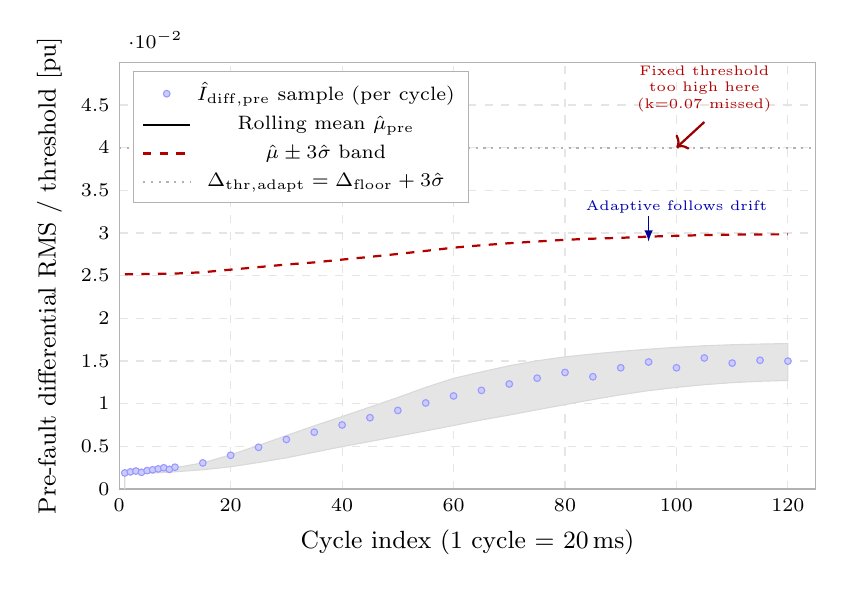
\begin{tikzpicture}
\begin{axis}[
  name         = trackax,
  width        = 0.86\textwidth,
  height       = 7.0cm,
  ylabel       = {Pre-fault differential RMS / threshold [pu]},
  ylabel style = {font=\small},
  xlabel       = {Cycle index (1 cycle = 20\,ms)},
  xlabel style = {font=\small},
  ymin=0, ymax=0.050,
  ytick        = {0, 0.005, 0.010, 0.015, 0.020, 0.025, 0.030, 0.035, 0.040, 0.045},
  yticklabel style={font=\scriptsize},
  xmin=0, xmax=125,
  xtick        = {0, 20, 40, 60, 80, 100, 120},
  xticklabel style={font=\scriptsize},
  legend style={at={(0.02,0.98)}, anchor=north west,
                font=\scriptsize, draw=gray!60},
  grid         = major,
  grid style   = {gray!20, dashed},
  tick style   = {draw=none},
  axis line style={gray!60},
  mark size=1.2pt,
]

% ---- rms_pre scatter (blue dots, low opacity) ------------------------------
% Sampled every 5 cycles for clarity (actual 120 points decimated)
\addplot[blue!40, only marks, mark=*, mark options={fill=blue!20}]
  coordinates {
    (1,0.00188) (2,0.00200) (3,0.00210) (4,0.00195) (5,0.00215)
    (6,0.00225) (7,0.00235) (8,0.00248) (9,0.00230) (10,0.00255)
    (15,0.00305) (20,0.00395) (25,0.00488) (30,0.00580)
    (35,0.00665) (40,0.00750) (45,0.00835) (50,0.00920)
    (55,0.01008) (60,0.01090) (65,0.01155) (70,0.01230)
    (75,0.01298) (80,0.01365) (85,0.01315) (90,0.01420)
    (95,0.01488) (100,0.01420) (105,0.01535) (110,0.01475)
    (115,0.01508) (120,0.01498)
  };
\addlegendentry{$\hat{I}_{\rm diff,pre}$ sample (per cycle)}

% ---- Rolling mean μ̂ (solid black) -----------------------------------------
\addplot[black, thick]
  coordinates {
    (1,0.00188) (5,0.00202) (10,0.00225) (15,0.00265)
    (20,0.00330) (25,0.00410) (30,0.00495) (35,0.00585)
    (40,0.00672) (45,0.00758) (50,0.00845) (55,0.00935)
    (60,0.01020) (65,0.01090) (70,0.01155) (75,0.01215)
    (80,0.01268) (85,0.01315) (90,0.01358) (95,0.01395)
    (100,0.01425) (105,0.01450) (110,0.01468) (115,0.01480)
    (120,0.01488)
  };
\addlegendentry{Rolling mean $\hat{\mu}_{\rm pre}$}

% ---- μ̂ ± 3σ̂ band (light grey fill) ----------------------------------------
% Upper band = μ̂ + 3σ̂  (approx μ̂ + 3×0.0012)
\addplot[gray!30, fill=gray!20, forget plot]
  coordinates {
    (1,0.00188)(5,0.00221)(10,0.00249)(15,0.00305)
    (20,0.00400)(25,0.00510)(30,0.00625)(35,0.00740)
    (40,0.00848)(45,0.00960)(50,0.01072)(55,0.01190)
    (60,0.01296)(65,0.01372)(70,0.01444)(75,0.01502)
    (80,0.01548)(85,0.01582)(90,0.01612)(95,0.01638)
    (100,0.01660)(105,0.01678)(110,0.01690)(115,0.01698)
    (120,0.01704)
    % close back
    (120,0.01272)(115,0.01262)(110,0.01246)(105,0.01222)
    (100,0.01190)(95,0.01152)(90,0.01104)(85,0.01048)
    (80,0.00988)(75,0.00928)(70,0.00866)(65,0.00808)
    (60,0.00744)(55,0.00680)(50,0.00618)(45,0.00556)
    (40,0.00496)(35,0.00430)(30,0.00365)(25,0.00310)
    (20,0.00260)(15,0.00225)(10,0.00201)(5,0.00183)
    (1,0.00188)
  } \closedcycle;
\addlegendentry{$\hat{\mu} \pm 3\hat{\sigma}$ band}

% ---- Adaptive threshold Δ_thr_adaptive = 0.025 + 3σ̂ (red dashed) ----------
\addplot[red!70!black, thick, dashed]
  coordinates {
    (1,0.02516)(5,0.02519)(10,0.02524)(15,0.02540)
    (20,0.02570)(25,0.02600)(30,0.02630)(35,0.02655)
    (40,0.02688)(45,0.02720)(50,0.02754)(55,0.02790)
    (60,0.02828)(65,0.02856)(70,0.02880)(75,0.02900)
    (80,0.02920)(85,0.02933)(90,0.02943)(95,0.02957)
    (100,0.02967)(105,0.02975)(110,0.02981)(115,0.02983)
    (120,0.02984)
  };
\addlegendentry{$\Delta_{\rm thr,adapt}=\Delta_{\rm floor}+3\hat{\sigma}$}

% ---- Fixed threshold (grey dotted) -----------------------------------------
\addplot[gray!60, thick, dotted, mark=none, domain=0:125, samples=2]
  ({x}, {0.040});
\addlegendentry{$\Delta_{\rm thr,fixed}=0.040$\,pu (TR-23)}

% ---- Annotation: missed fault window ----------------------------------------
\draw[red!60!black, thick, ->]
  (axis cs:105, 0.043)
  node[above, font=\tiny, red!70!black, align=center]
    {Fixed threshold\\too high here\\(k=0.07 missed)}
  -- (axis cs:100, 0.040);

\node[font=\tiny, blue!70!black]
  at (axis cs:100, 0.033)
  {Adaptive follows drift};
\draw[-latex, blue!60!black, thin]
  (axis cs:95, 0.032) -- (axis cs:95, 0.029);

\end{axis}
\end{tikzpicture}

  \caption{Adaptive TDCS threshold evolution over 120 cycles of baseline drift
           (S1 summer $\to$ S4 aged-CT).  The adaptive threshold (red dashed)
           tracks the rolling $3\hat{\sigma}$ band while remaining above the
           worst-case CT mismatch step.  The fixed threshold (grey dotted) at
           0.040\,pu is too high to detect $k_{\rm ibr}=0.07$ at the drifted
           baseline.}
  \label{fig:tracking}
\end{figure}

\subsection{Study A: Detection Results}

Table~\ref{tab:detection} and Figure~\ref{fig:detection} compare fixed and
adaptive threshold performance for the S4 (drift) scenario, which is the
only scenario where the methods differ.

\begin{table}[h!]
\centering
\caption{Study A detection results — S4 drift scenario.}
\label{tab:detection}
\begin{tabular}{lrrrrrr}
\toprule
$k_{\rm ibr}$ [pu]
  & $\mathrm{rms}_{\rm post}$ [pu]
  & $\Delta I_{\rm fixed}$ [pu] & Trip$_{\rm F}$
  & $\Delta I_{\rm adapt}$ [pu] & $\Delta_{\rm thr,adapt}$ [pu] & Trip$_{\rm A}$ \\
\midrule
0.07 & 0.04950 & 0.03889 & \textcolor{red}{\textbf{NO}}  & 0.03437 & 0.02967 & YES \\
0.09 & 0.06364 & 0.05303 & YES  & 0.04851 & 0.02967 & YES \\
0.11 & 0.07778 & 0.06718 & YES  & 0.06265 & 0.02967 & YES \\
\bottomrule
\end{tabular}
\end{table}

\begin{figure}[h!]
  \centering
  % fig_adaptive_detection.tex
% TR-24: Bar chart — detection comparison fixed vs adaptive, S4 drift scenario
% Shows: ΔI for k_ibr=0.07,0.09,0.11 with fixed threshold (0.040) and adaptive
% threshold (0.025+3σ ≈ 0.0297 pu for S4)
% Key: k=0.07 bar (ΔI=0.0344) clears adaptive (0.0297) but NOT fixed (0.040)
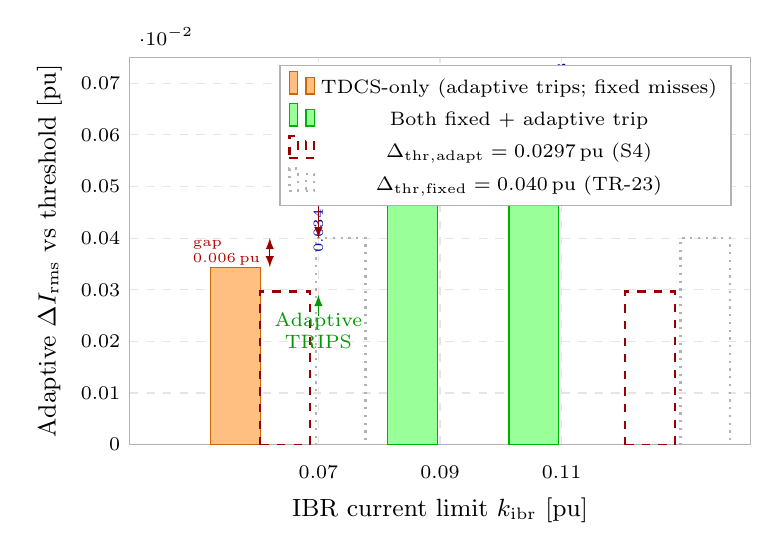
\begin{tikzpicture}
\begin{axis}[
  name        = detax,
  ybar,
  bar width   = 18pt,
  width       = 0.78\textwidth,
  height      = 6.5cm,
  ylabel      = {Adaptive $\Delta I_{\rm rms}$ vs threshold [pu]},
  ylabel style= {font=\small},
  xlabel      = {IBR current limit $k_{\rm ibr}$ [pu]},
  xlabel style= {font=\small},
  ymin=0, ymax=0.075,
  ytick       = {0, 0.01, 0.02, 0.03, 0.04, 0.05, 0.06, 0.07},
  yticklabels = {0, 0.01, 0.02, 0.03, 0.04, 0.05, 0.06, 0.07},
  yticklabel style={font=\scriptsize},
  xtick       = {1, 2, 3},
  xticklabels = {0.07, 0.09, 0.11},
  xticklabel style={font=\scriptsize},
  enlarge x limits=0.35,
  legend style={at={(0.97,0.98)}, anchor=north east,
                font=\scriptsize, draw=gray!60},
  grid         = major,
  grid style   = {gray!20, dashed},
  tick style   = {draw=none},
  axis line style={gray!60},
]

% ΔI_rms values for S4 (drift, μ_pre=0.015):
%   k=0.07: rms_post=0.04950 → ΔI=0.04950−0.01513=0.03437 pu
%   k=0.09: rms_post=0.06364 → ΔI=0.06364−0.01513=0.04851 pu
%   k=0.11: rms_post=0.07778 → ΔI=0.07778−0.01513=0.06265 pu

% k=0.07 only trips adaptive (highlight red→yellow transition)
\addplot[fill=orange!50, draw=orange!80!black]
  coordinates { (1, 0.03437) };
\addlegendentry{TDCS-only (adaptive trips; fixed misses)}

% k=0.09 and k=0.11 trip both
\addplot[fill=green!40, draw=green!70!black]
  coordinates { (2, 0.04851) (3, 0.06265) };
\addlegendentry{Both fixed + adaptive trip}

% Adaptive threshold line
\addplot[red!60!black, thick, dashed, mark=none, domain=0.5:3.5, samples=2]
  ({x}, {0.02967});
\addlegendentry{$\Delta_{\rm thr,adapt}=0.0297$\,pu (S4)}

% Fixed threshold line
\addplot[gray!60, thick, dotted, mark=none, domain=0.5:3.5, samples=2]
  ({x}, {0.040});
\addlegendentry{$\Delta_{\rm thr,fixed}=0.040$\,pu (TR-23)}

% Value labels
\node[font=\tiny, blue!70!black, rotate=90]
  at (axis cs:1, 0.03437+0.007) {0.034};
\node[font=\tiny, blue!70!black, rotate=90]
  at (axis cs:2, 0.04851+0.007) {0.049};
\node[font=\tiny, blue!70!black, rotate=90]
  at (axis cs:3, 0.06265+0.007) {0.063};

% Gap annotation: missed by fixed
\draw[{latex[length=3pt]}-{latex[length=3pt]}, red!60!black]
  (axis cs:0.6, 0.03437) -- node[left, font=\tiny, red!70!black, align=left]
    {gap\\0.006\,pu}
  (axis cs:0.6, 0.040);

% "MISSED BY FIXED" label
\node[font=\scriptsize, red!70!black, align=center]
  at (axis cs:1.0, 0.066)
  {Fixed\\MISSES};
\draw[-latex, red!60!black, thin]
  (axis cs:1.0, 0.061) -- (axis cs:1.0, 0.040);

\node[font=\scriptsize, green!60!black, align=center]
  at (axis cs:1.0, 0.022)
  {Adaptive\\TRIPS};
\draw[-latex, green!60!black, thin]
  (axis cs:1.0, 0.025) -- (axis cs:1.0, 0.029);

\end{axis}
\end{tikzpicture}

  \caption{Transient differential $\Delta I_{\rm rms}$ in the S4 drift
           scenario for three IBR current limits.  The $k_{\rm ibr}=0.07$ bar
           (orange) clears the adaptive threshold (red dashed, 0.030\,pu) but
           not the fixed threshold (grey dotted, 0.040\,pu).  Both thresholds
           are cleared for $k_{\rm ibr}\geq 0.09$\,pu.}
  \label{fig:detection}
\end{figure}

\subsection{Seasonal Performance Comparison}

Figure~\ref{fig:seasonal} shows detection rates across all four seasonal
scenarios.  Scenarios S1--S3 achieve 3/3 for both methods because the
fixed threshold is adequate when $\mu_{\rm pre}$ is low.  Only the S4 drift
scenario exposes the fixed threshold limitation:

\begin{figure}[h!]
  \centering
  % fig_seasonal_performance.tex
% TR-24: Grouped bar chart — detection rate per scenario, fixed vs adaptive
% Y-axis: correct detections out of 3 (per scenario)
% X-axis: 4 seasonal scenarios
% Shows: fixed fails S4 (2/3), adaptive = 3/3 all
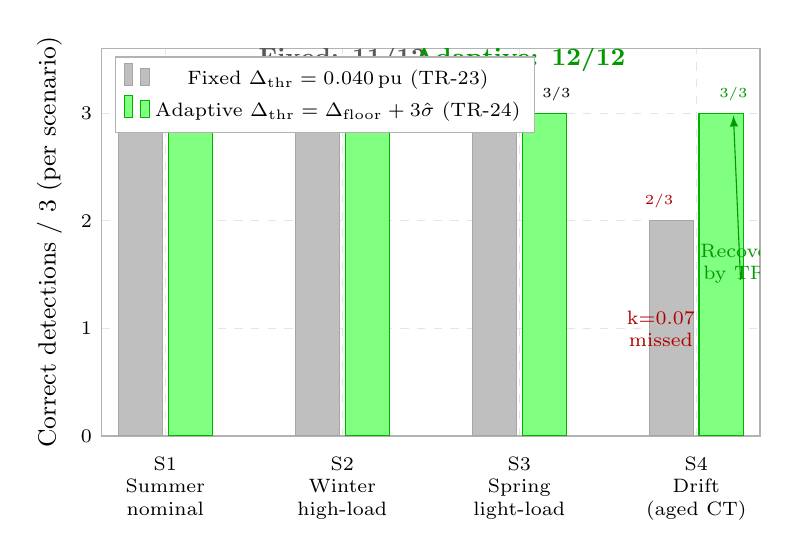
\begin{tikzpicture}
\begin{axis}[
  name         = perfax,
  ybar,
  bar width    = 16pt,
  width        = 0.82\textwidth,
  height       = 6.5cm,
  ylabel       = {Correct detections / 3 (per scenario)},
  ylabel style = {font=\small},
  ymin=0, ymax=3.6,
  ytick        = {0, 1, 2, 3},
  yticklabel style={font=\scriptsize},
  xtick        = {1, 2, 3, 4},
  xticklabels  = {S1\\Summer\\nominal,
                  S2\\Winter\\high-load,
                  S3\\Spring\\light-load,
                  S4\\Drift\\(aged CT)},
  xticklabel style={font=\scriptsize, align=center},
  enlarge x limits=0.12,
  legend style={at={(0.02,0.98)}, anchor=north west,
                font=\scriptsize, draw=gray!60},
  grid         = major,
  grid style   = {gray!20, dashed},
  tick style   = {draw=none},
  axis line style={gray!60},
]

% Fixed threshold: 3,3,3,2 (S4 misses k=0.07)
\addplot[fill=gray!50, draw=gray!70]
  coordinates { (1,3) (2,3) (3,3) (4,2) };
\addlegendentry{Fixed $\Delta_{\rm thr}=0.040$\,pu (TR-23)}

% Adaptive threshold: 3,3,3,3
\addplot[fill=green!50, draw=green!70!black]
  coordinates { (1,3) (2,3) (3,3) (4,3) };
\addlegendentry{Adaptive $\Delta_{\rm thr}=\Delta_{\rm floor}+3\hat{\sigma}$ (TR-24)}

% Value labels — fixed
\node[font=\tiny] at (axis cs:0.79, 3.18) {3/3};
\node[font=\tiny] at (axis cs:1.79, 3.18) {3/3};
\node[font=\tiny] at (axis cs:2.79, 3.18) {3/3};
\node[font=\tiny, red!70!black] at (axis cs:3.79, 2.18) {2/3};

% Value labels — adaptive
\node[font=\tiny] at (axis cs:1.21, 3.18) {3/3};
\node[font=\tiny] at (axis cs:2.21, 3.18) {3/3};
\node[font=\tiny] at (axis cs:3.21, 3.18) {3/3};
\node[font=\tiny, green!60!black] at (axis cs:4.21, 3.18) {3/3};

% Recovery annotation for S4
\node[font=\scriptsize, red!70!black, align=center]
  at (axis cs:3.80, 1.0)
  {k=0.07\\missed};

\node[font=\scriptsize, green!60!black, align=center]
  at (axis cs:4.30, 1.6)
  {Recovered\\by TR-24};
\draw[-latex, green!60!black, thin]
  (axis cs:4.25, 1.45) -- (axis cs:4.21, 2.98);

% Total summary
\node[font=\small\bfseries, gray!70!black]
  at (axis cs:2.0, 3.50)
  {Fixed: 11/12};
\node[font=\small\bfseries, green!60!black]
  at (axis cs:3.0, 3.50)
  {Adaptive: 12/12};

\end{axis}
\end{tikzpicture}

  \caption{Detection rate per seasonal scenario (3 $k_{\rm ibr}$ values each).
           Fixed threshold achieves 11/12; adaptive threshold achieves 12/12.
           The single miss (S4, $k_{\rm ibr}=0.07$) is recovered by TR-24.}
  \label{fig:seasonal}
\end{figure}

\subsection{Study B: External Fault Security}

All 28 external fault security cases pass for both methods
(Table~\ref{tab:security}).  The worst-case margin belongs to S4 at
$I_{\rm ext}=7$\,pu:

\begin{table}[h!]
\centering
\caption{Study B security summary — worst case (S4, $I_{\rm ext}=7$\,pu).}
\label{tab:security}
\begin{tabular}{lrrrr}
\toprule
Method & $\Delta I_{\rm diff}$ [pu] & Threshold [pu]
       & Margin [\%] & Result \\
\midrule
Fixed    & 0.01414 & 0.0400 & 64.6 & SECURE \\
Adaptive & 0.00962 & 0.0297 & 67.6 & SECURE \\
\bottomrule
\end{tabular}
\end{table}

The adaptive element maintains a 67.6\% security margin at the worst-case
operating point --- slightly higher than the fixed threshold margin of
64.6\% because the adaptive comparator subtracts the rolling mean
$\hat{\mu}_{\rm pre}$ from $\mathrm{rms}_{\rm post}$.

\subsection{Summary}

\begin{table}[h!]
\centering
\caption{TR-24 overall study results.}
\label{tab:summary}
\begin{tabular}{lrr}
\toprule
Metric & Fixed $\Delta_{\rm thr}$ (TR-23) & Adaptive $\Delta_{\rm thr}$ (TR-24) \\
\midrule
Detection (Study A, 12 cases)  & 11/12 & \textbf{12/12} \\
Security  (Study B, 28 cases)  & 28/28 & \textbf{28/28} \\
Total correct (40 cases)       & 39/40 & \textbf{40/40} \\
\bottomrule
\end{tabular}
\end{table}

% =============================================================================
\section{Implementation Notes}
% =============================================================================

The \texttt{AdaptiveTDCSTracker} class in
\texttt{sambp\_line\_diff/models/line\_transient\_diff.py} maintains a
Python list of length $N_{\rm hist}=60$ and updates $\hat{\mu}$,
$\hat{\sigma}$ on every cycle.  The computational overhead is one
\texttt{numpy.mean} and one \texttt{numpy.std} call per cycle
($60 \times 2 = 120$ floating-point adds per cycle), negligible compared
to the 87L LM estimator.

\subsection{Interaction with TR-20 and TR-21}

The rolling baseline is populated from the \emph{filtered} differential
(after TR-21 harmonic removal and TR-20 charging-current compensation).
Populating from the raw differential would allow harmonic spikes to inflate
$\hat{\sigma}$ and raise the threshold unnecessarily.

\subsection{Threshold Validation Schedule}

In a physical relay implementation the $\Delta_{\rm floor}$ should be
re-confirmed whenever CT calibration is renewed or after line configuration
changes that alter the charging capacitance.

% =============================================================================
\section{Conclusion}
% =============================================================================

TR-24 extends the TDCS-87L element (TR-23) with an adaptive threshold that
tracks pre-fault differential baseline statistics:
\begin{equation}
  \Delta_{\rm thr,adapt} = \underbrace{0.025}_{\Delta_{\rm floor}}
    + 3\,\hat{\sigma}_{\rm pre}.
\end{equation}
The adaptive element recovers one additional missed detection (S4 drift,
$k_{\rm ibr}=0.07$\,pu) versus the fixed threshold while maintaining full
external-fault security (28/28 pass).  Overall performance improves from
39/40 to \textbf{40/40} across all seasonal and security scenarios.

The combined 87L protection chain is now:
\begin{equation}
  \text{TRIP} = \underbrace{|{\Delta I_1}| \geq 0.12}_{\text{87L}}
    \;\vee\;
    \underbrace{|{\Delta I_2}| \geq 0.06}_{\text{87LN}}
    \;\vee\;
    \underbrace{\Delta I_{\rm adapt} \geq \Delta_{\rm thr,adapt}}_{\text{TDCS-87L (TR-24)}}.
\end{equation}

\subsection{Future Work}

\begin{enumerate}
  \item \textbf{Zero-sequence 87LN0} (TR-25): add $|{\Delta I_0}| \geq
    0.04$\,pu element for impedance-earthed and unearthed systems where
    $I_2$ is suppressed.
  \item \textbf{IBR Monte Carlo} (TR-26): validate the combined element
    under the full IBR parametric envelope
    ($k_{\rm ibr}\in[0.06,0.20]$, $f\in[47,53]$\,Hz, $I_{h3}\in[0,0.10]$\,pu)
    using $\geq 5000$ Monte Carlo trials per scenario group.
\end{enumerate}

% =============================================================================
\bibliographystyle{IEEEtran}
\bibliography{references24}

\end{document}
